\documentclass[a4paper]{article}

% natbib
\usepackage[numbers,sort]{natbib}

\usepackage{mysimpletemplatewn}
\usepackage[utf8]{inputenc} %%% to support copy and paste with accents for french stuff
\usepackage[T1]{fontenc} %%%key to get copy and paste for the code!
\usepackage{times}
\usepackage[french]{babel}
\usepackage[scaled=0.85]{helvet}
\usepackage{graphicx}
\usepackage{ifthen}
\usepackage{xspace}
\usepackage{alltt}
\usepackage{latexsym}
\usepackage{url}
\usepackage{amsmath,amssymb,amsfonts}
\usepackage{stmaryrd}
\usepackage{algorithmic}
\usepackage{textcomp}
\usepackage{xcolor}
\usepackage{enumerate}
% \usepackage{cite}
\usepackage[pdftex,colorlinks=true,pdfstartview=FitV,linkcolor=blue,citecolor=blue,urlcolor=blue]{hyperref}
\usepackage{multirow}
\usepackage{listings}
\usepackage{color}
\usepackage{subcaption}

\usepackage{pgfgantt}

\usepackage{bibentry}
\nobibliography*


\newboolean{showcomments}
\setboolean{showcomments}{true}
\ifthenelse{\boolean{showcomments}}
  {\newcommand{\bnote}[2]{
	\fbox{\bfseries\sffamily\scriptsize#1}
    {\sf\small$\blacktriangleright$\textit{#2}$\blacktriangleleft$}
    % \marginpar{\fbox{\bfseries\sffamily#1}}
   }
   \newcommand{\paragraphDesc}[2]{
    \textcolor{#1}{#2}
   }
   
  }
  {\newcommand{\bnote}[2]{}
   \newcommand{\cvsversion}{}
   \newcommand{\paragraphDesc}[2]{}
  }

\newcommand{\here}{\bnote{***}{CONTINUE HERE}}
\newcommand{\nb}[1]{\bnote{NB}{#1}}

\newcommand{\fix}[1]{\bnote{FIX}{#1}}
%%%% add your own macros 


\newcommand{\sd}[1]{\bnote{Stef}{\textcolor{orange}{#1}}}
\newcommand{\an}[1]{\bnote{Anne}{\textcolor{green}{#1}}}
\newcommand{\bv}[1]{\bnote{Benoit}{\textcolor{blue}{#1}}}
\newcommand{\nic}[1]{\bnote{Nic}{\textcolor{red}{#1}}}

\newcommand{\todo}[1]{\bnote{TODO}{#1}}

\graphicspath{{figures/}}
%%% 


\newcommand{\figref}[1]{Figure~\ref{fig:#1}}
\newcommand{\figlabel}[1]{\label{fig:#1}}
\newcommand{\tabref}[1]{Table~\ref{tab:#1}}
\newcommand{\layout}[1]{#1}
\newcommand{\commented}[1]{}
\newcommand{\secref}[1]{Section~\ref{sec:#1}}
\newcommand{\seclabel}[1]{\label{sec:#1}}

%\newcommand{\ct}[1]{\textsf{#1}}
\newcommand{\stCode}[1]{\textsf{#1}}
\newcommand{\stMethod}[1]{\textsf{#1}}
\newcommand{\sep}{\texttt{>>}\xspace}
\newcommand{\stAssoc}{\texttt{->}\xspace}

\newcommand{\stBar}{$\mid$}
\newcommand{\stSelector}{$\gg$}
\newcommand{\ret}{\^{}}
\newcommand{\msup}{$>$}
%\newcommand{\ret}{$\uparrow$\xspace}

\newcommand{\myparagraph}[1]{\noindent\textbf{#1.}}
\newcommand{\eg}{\emph{e.g.}\xspace}
\newcommand{\ie}{\emph{i.e.}\xspace}
\newcommand{\etal}{\emph{et al.,}\xspace}
\newcommand{\ct}[1]{{\textsf{#1}}\xspace}
\newcommand{\etc}[1]{\textit{etc.}}



\newcommand{\defaultScale}{0.55}
\newcommand{\pic}[3]{
   \begin{figure}[h]
   \begin{center}
   \includegraphics[scale=\defaultScale]{#1}
   \caption{#2}
   \label{#3}
   \end{center}
   \end{figure}
}


\newcommand{\twocolumnpic}[3]{
  \begin{figure*}[!ht]
  \begin{center}
  \includegraphics[scale=\defaultScale]{#1}
  \caption{#2}
  \label{#3}
  \end{center}
  \end{figure*}
}

\newcommand{\picw}[3]{
  \begin{figure}[htbp]
  \begin{center}
  \includegraphics[width=\columnwidth]{#1}
  \caption{#2}
  \label{#3}
  \end{center}
  \end{figure}
}


\newcommand{\infe}{$<$}
\newcommand{\supe}{$\rightarrow$\xspace}
\newcommand{\di}{$\gg$\xspace}
\newcommand{\adhoc}{\textit{ad-hoc}\xspace}

\usepackage{url}            
\makeatletter
\def\url@leostyle{%
  \@ifundefined{selectfont}{\def\UrlFont{\sf}}{\def\UrlFont{\small\sffamily}}}
\makeatother
% Now actually use the newly defined style.
\urlstyle{leo}

\definecolor{codegreen}{rgb}{0,0.6,0}
\definecolor{codegray}{rgb}{0.5,0.5,0.5}
\definecolor{codepurple}{rgb}{0.58,0,0.82}
\definecolor{backcolour}{rgb}{0.95,0.95,0.92}

\lstdefinestyle{mystyle}{
    backgroundcolor=\color{backcolour},
    commentstyle=\color{codegreen},
    keywordstyle=\color{magenta},
    numberstyle=\tiny\color{codegray},
    stringstyle=\color{codepurple},
    basicstyle=\footnotesize,
    breakatwhitespace=false,
    breaklines=true,
    captionpos=b,
    keepspaces=true,
    numbers=left,
    numbersep=5pt,
    showspaces=false,
    showstringspaces=false,
    showtabs=false,
    tabsize=2
}

\lstset{style=mystyle}
\newcommand{\browserMaster}{\textit{BrowserMaster} \xspace}

\title{CST --Analyse multi-facettes et opérationnelle pour la transformation des systemes d’information}
\author{ HOUEKPETODJI Mahugnon Honoré}

\begin{document}

\institution{}

\date{\today}

\maketitle

% \begin{abstract}
% The abstract text goes here.
% \end{abstract}
\section{Description du sujet de la thèse}
% 0.5 (1/2) pages
CIM est une SAS au capital social de 200 k détenu à 100\% par DL Software. 
CIM est éditeur, intégrateur, hébergeur et infogéreur de solutions pour l'assurance de personnes en santé, prévoyance. 
Elle offre une expertise Santé et Prévoyance acquise après plus de 30 ans auprès de ses clients. 
CIM est hébergeur de ses solutions pour 90\% de ses clients et plus de 1000 utilisateurs. 
Toutes les thématiques d'infrastructure et de surveillance des flux sont intégrées à cette offre.
CIM est propriétaire de ses infrastructures serveurs, tous les éléments actifs des systèmes et tous les éléments de stockage sont achetés par CIM, gérés et supervisés par les équipes de CIM. Aucun sous-traitant n'intervient dans les opérations quotidiennes d'hébergement, d'exploitation des solutions et des données hébergées.

CIM est certifiée \textit{Microsoft GOLD Partner}. 
Elle est l'éditeur des progiciels de la gamme Izy Links et assure l'intégration de l'ensemble des briques de cette gamme ainsi que des briques partenaires nécessaires à la bonne réussite du projet. Cette solution est développée en PowerBuilder sur base de données DB2.
L'équipe de développement vient d'avoir PowerBuilder version 2017 (été 2018) et est en cours de passage sur DB2 v11.

Le système de gestion est centré sur Izy Protect, autour duquel gravite l'ensemble des briques complémentaires répondant à l'assemble des besoins, et pouvant être activées ou non. 
La société CIM a effectué une analyse de risque pour son évolution et croissance en 2017 d'où il ressort que Izy Protect souffre des problèmes 
(1) Vieux langage,
(2) Logiciel vieillissant,
(3) Perte savoir,
(4) Changements à haut risque.
Ces problèmes sont récurrents chez les organismes gérant des systèmes d'information \cite{Deme02a}.

Ce travail de doctorat consiste à proposer des modèles et des mécanismes permettant d'assurer une ré-ingénierie des systèmes d'information. 
Les expériences et validation des prototypes se feront dans le contexte de l'application du système d'information écrit en PowerBuilder de la société CIM


\section{Etat de l'art}
\label{sec:stateOfTheArt}
% 1 pages
Dans cette section, je presenterai Izy Protect et les travaux qui se penchent sur la question de la ré-ingénierie des systèmes d'informations.
%===========================================================================================================================================================
\subsection{Présentation de Izy Protect}
\label{sec:izyProtect}
Izy Protect est un système de plus de 3 MLOC écrit en Powerbuilder et maintenu depuis plus de 20 ans par les développeurs de la CIM. 
Aujourd'hui Izy Protect est maintenu par une equipe de 18 developpeurs.
 Le code source est organisé par bibliothèques Powerbuilder. 
Izy Protect compte 117 bibliothèques. Les bibliothèques de Izy Protect peuvent être regroupées en des modules métier.
 Par contre cette information ne peux pas être directement déduites du code.
 La plus large à une taille d'environ 300 KLOC.
Durant toutes ces années, il y a eu beaucoup de changement dans l'équipe de développeurs. 
Vu la complexité actuelle du système, les développeurs ont de plus en plus du mal à le maintenir.
Les anciennes versions du système sont stockées sur un disque dur.
 Pour des raisons internes à la CIM, les versions d'Izy Protect ont été perdues jusqu'en 2010. 
 De plus, les développeurs risquent à tout moment de faire de régression (casser une fonctionnalité existant). 
Izy Protect  n'est pas couvert avec des tests unitaires automatisés.
Ceci augmente la craint des développeurs pour de petites modifications. 
Les caractéristiques de Izy Protect montre qu'il est un système de valeur pour l'entreprise. En plus il est développé avec un vieux langage de programmation: PowerBuilder.
Ces caractéristiques reflètent la définition d'un système \textbf{patrimonial} selon \citet{Deme02a}.
De plus, quand un système a plusieurs décennies de vie, la rétro-ingénierie est une activité centrale pour le maintenir \cite{Deme02a}.

Dans l'entreprise, les travaux de maintenances ou de developpements sur Izy Protect sont identifiés par des tickets.
Les tickets sont stockés dans la base de données des tickets ou fiches navettes depuis 1998. 
La base de données des tickets pilote l'ensemble du processus d'évolution du logiciel : attribution du travail aux développeurs, gestion du flux de travail pour répondre à une demande du client, informations de facturation sur chaque tâche.
Il existe des tickets pour la correction de défauts, la rédaction de documentation, l'ajout de nouvelles fonctionnalités, etc. 

Un ticket comporte entre autres les caractéristiques suivantes :

\begin{itemize}
\item la date de création
\item la date de clôture
\item l'estimation du temps nécessaire au développeur pour travailler sur le ticket
\item temps passé par un développeur
\begin{itemize}
\item le temps d'analyser
\item le temps de mettre en œuvre une solution
\item le temps de test
\end{itemize}
\item le(s) bibliothèque(s) impactée(es)
\end{itemize}


\subsection{Analyse de l'évolution de l'état d'un système logiciel patrimonial}
\label{sec:etatLogiciel}
Les systèmes patrimoniaux sont des systèmes en constant changement : production de nouvelles fonctionnalités.
La deuxième loi de Lehman \cite{Lehm96a} stipule qu'à mesure que les logiciels évoluent, la complexité croissante et l'augmentation des défauts entraîneront une baisse de la satisfaction des parties prenantes, à moins que les équipes de projet n'entreprennent le travail nécessaire pour maintenir la qualité.
Selon \citet{Deme02a}, collecter et interpréter les données et les résumer dans une vue cohérente est une étape importante pour la compréhension initiale d'un système logiciel existant.
Dans ce sens, de nombreux travaux de la littérature proposent des techniques, pour suivre l'évolution de l'état de ces systèmes.

\citet{Zhan10b} utilise les données des occurrences bugs et le temps pour modéliser l'évolution d'un système logiciel avec c\-charts.

\citet{lenar17} propose un système de recommandation d'action au développeur pour un nouveau bug. Le système se base sur l'historique des bugs, le code source ainsi que qu'un algorithme de prédiction. Pour que ça marche, le code source doit être géré dans un système de contrôle de version. Ce qui n'est pas le cas avec Izy Protect.

\citet{port17} utilise les modèles et l'analyse de l'historique des défauts pour évaluer la qualité d'un système et prédire l'effort nécessaire pour améliorer le système. Les métriques mesurées sont : le taux de bugs sur une période de temps, le ratio entre le taux de d'augmentation de la taille du système et le taux de bugs, le temps moyen entre la découverte des bugs, l'effort pour résoudre les bugs, estimation des risques de futurs bugs...
Certain de ces métriques comme : le taux de bugs par période de temps, l'effort pour résoudre les bugs sont intéressants dans le cadre d'Izy Protect. 
Les autres ne se conforment pas au contexte, car les tickets d'Izy protect ne sont directement liés au code de façon standard.
Chaque développeur note le numéro de tickets à sa façon dans le code. 


\citet{kim07,Bibi06} proposent des modèles de prédiction des défauts avec des algorithmes d'apprentissage en utilisant l'historique des bugs de système. 
Les algorithmes de prédiction de bugs ne sont pas toujours consistants \cite{bang19}. De plus, ils ne tiennent pas compte des changements qui peuvent être imprévisible dans le code. De plus, Izy Protect est logiciel commercial, multi-utilisateurs, et donc chaque utilisateur a des fonctionnalités ou des changements qui lui est spécifique. 

\citet{naga05} utilise l'historique le nombre de lignes de code changées pour une correction de  bug  ou une nouvelle fonctionnalité pour prédire la densité de bug le code. Pour que ceci soit réalisable, il faut que le code soit préalablement versionné dans un système de contrôle de version.

\citet{Raja09} à étudier différents algorithme de modélisation des défauts d'un système à partir des donnée des défauts relevés sur huit projets dont les codes sources sont ouverts. Il en ressort que la moyenne glissée modélise mieux les défauts des systèmes.

\subsection{Rétro-ingénierie}
\label{sec:retroingenierie}
Dans cette section, je présenterai les travaux reliés à l'outillage pour la rétro-ingénierie que j'ai étudié.
\citet{Chik90a} définit la rétro-ingénierie comme \textit{un processus d'analyse d'un système données pour identifier les composants du système et leurs relations, afin de créer des représentations du système sous une autre forme ou à un niveau d'abstraction plus élevé."}.

\citet{Brun14c} affirme que la rétro-ingénierie n'est pas limitée à certains langages courants, mais est universelle. 
Par exemple, elle peut concerner la base de données \cite{Delp20a} ou l'interface graphique \cite{Verh19a}.
Il est donc nécessaire de disposer d'une suite d'outils polyvalents et extensibles, indépendants du langage : cette extension peut se faire à plusieurs niveaux - méta-modèle.
Mais aussi au niveau des outils eux-mêmes (par exemple en agissant sur le modèle).

C'est dans cette optique que \citet{Kien10a} reconnaissent  le besoin d'outils pour la retro-ingénierie qui fournissent des fonctionnalités permettant d'extraire des informations de bas niveau des systèmes, d'analyser et de générer des connaissances sur les systèmes, et de visualiser ces connaissances afin que les ingénieurs puissent comprendre efficacement les aspects du système qui les intéressent.
De ce point de vue ils identifient que ces outils doivent être:

  (1) scalable: capacité de ces outils a fonctionné pour la rétro-ingénierie de petites aux larges logiciels;
  (2) interoperable: ces outils doivent être capital de Communiquer avec des outils externes;
 (3) personnalisable: les activités de rétro-ingénierie étant variables, les utilisateurs d'outils de retro-ingenierie doivent pouvoir continuellement
 les  adapter pour répondre aux besoins changeants;
 (4) utilisable: facilité d'utilisation;
(5) adoptable: facilité d'apprentissage.

Ainsi les outils qui seront proposés pour la rétro-ingénierie de Izy Protect doivent respecter ces règles là.

\citet{Bell98a} ont proposé un esemble de critères pour comparer les outils de rétro-ingénierie.
Par contre, ils ne couvrent pas le méta-modèle, l'extension du méta-modèle et des outils de manière exhaustive.

\citet{Govi18a} ont identifié des critères pour les outils de réingénierie. 
Parmi ces critères, j'ai retenu ceux qui se rapportent à la rétro-ingénierie.
Ce sont les critères (1) de sélection (2) d'abstraction.  
Le critère de sélection exige que l'outil de rétro-ingénierie permette a l'utilisateur de selectionner des éléments  du code source d'un système 
qui repondent à une requête donnée.
L'outil doit aussi permettre a l'utilisateur d'abstraire les caractéristiques des entités du code souce à un haut nivau d'abstraction. 
Par example: déduire de la complexité cyclomatique des classes d'un package, la complexité cyclomatique du package.


%Modisco
\citet{Brun14c} a proposé et mis en œuvre le cadre MoDisco.
MoDisco est divisé en 4 couches, un projet de modélisation de la plateforme Eclipse, l'infrastructure, la technologie et les cas d'utilisation.
La couche infrastructure contient des outils génériques permettant de naviguer et d'interroger les modèles.
La couche technologie contient le méta-modèle spécifique (Java, XML, JSP, ...).
Et la couche des cas d'utilisation contient l'action spécifique pour un modèle, par exemple le remaniement de code Java.
MoDisco inclut: un navigateur de modèle, un éditeur pour voir le code des entité d'un modèle, un support graphique pour faire des requêtes sur les éléments du modèle. 
Par contre \citet{Brun14c}, ne propose que l'UML pour visualiser les éléments d'un modèle.
Alors que pour un système large, l'UML devient vite une toile d'araignée et freine une compréhension rapide du système.

\section{Avancées actuelles}
% 3 pages
\subsection{Route vers le DevOps}
\label{sec: devOps}
Les problèmes préalablement cités sur Izy Protect à savoir : code non versionné, ce qui engendre les pertes et écrasement de code, puis l'absence total de test unitaire automatisé, m'ont amenés à :
\begin{itemize}
\item  Mettre en place un serveur  pour versionné le code. 
Le fait de versionné le code  non seulement permet d'eviter les problèmes de pertes de code mais aussi a longterme me permettrai
(1) d'avoir une base d'analyse de l'evolution du code de Izy Proctect suplemenetaire et (2) de fournire  un outils de vérification des normmes de developpements sur les changements effectués par les developpeurs.
 
J'ai choisi Subversion( SVN) \footnote{https://subversion.apache.org/} par le fait de sa simplicité pour la compréhension.
Il faut aussi noté que le module de contrôle de version qu'offre Powerbuilder n'est pas trop stable. 
Par exemple, parfois, le module considère un code déjà versionné comme un code non versionné.
De plus, le module de contrôle de version qu'offre Powerbuilder ne supporte pas bien les opérations avancées comme la comparaison de deux versions du code ou bien la résolution de conflit. 
Tout cela fait de SVN un choix simple pour commencer.
En complément de Powerbuilder, j'ai amené les développeurs de la CIM à utiliser TortoiseSVN\footnote{https://tortoisesvn.net/}.
Il faut signaler que pour le success de la mise en place, il a fallut une documentation et une assistance continue.

Dans le but d'avoir une base d'analyse de l'evolution du code de Izy Protect, reconstruire l'histoire du code source de Izy Protect depuis 2012 afin de procéder à des analyses de l'évolution du système à partir des changements entre les versions. 
Les versions d'Izy Protect sont nombreuses. J'en suis actuellement sur les versions produites en 2015.
\item Commencer la mise en place des tests automatisé.
 PBUnit\footnote{https://sourceforge.net/p/pbunit/wiki/Home/} qui paraît être la libraire qui permet de tester les fonctionnalités des applications Powerbuilder au niveau du code source. 

\end{itemize}

\subsection{Analyse des fiches navettes}
\label{sec:analyseDesFichesNavettes}
A travers l'analyse des tickets, j'espère  caracteriser l'état de Izy Protect avec des données factuelles, 
et suivre  les changements du système dans le temps.
Ceci permettra  d'evaluer l'impact de l'utilisation des outils d'aide à la rétro-ingénierie que je proposerai durant cette thèse.
Pour cela, j'ai utilisé la base de donnée des fiches navettes. 
Après nettoyage, seul les tickets à partir de 2004 sont utilisable. 
Les données sont non-stationnaires. 
En me basant sur les résultats de \cite{Raja09}, j'ai utilisé la moyenne glissant avant un pas de 2 mois pour modéliser l'état du système.
J'ai principalement mesuré les métriques suivantes : l'evolution du temps pour ferme les tickets, l'évolution du temps nécessaire aux développeurs, l'evolution du temps des tests manuel du developpeur, l'évolution de l'estimation du temps de développement par le manager.
Les résultats sont présentés dans un tableau de board qui se met à jours chaque mois.
La \figref{dashboardFig} montre l'aperçu du tableau de bord.
\begin{figure}[htbp]
  \begin{center}
  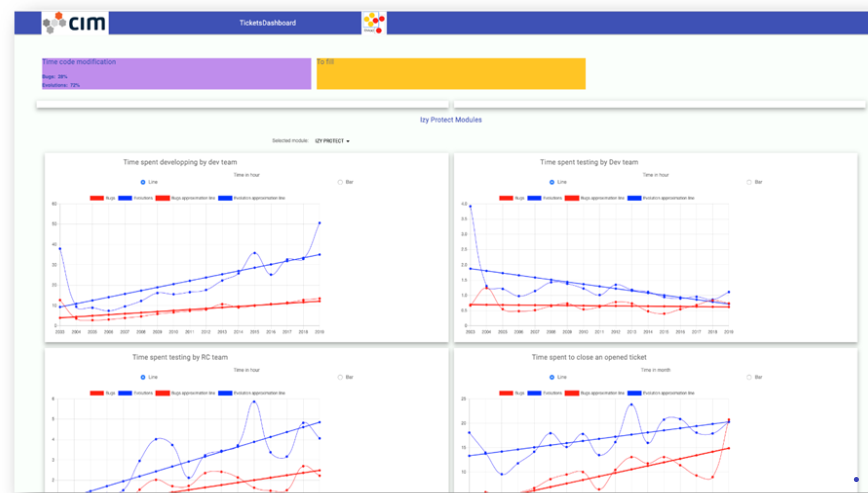
\includegraphics[width=0.8\textwidth]{./figures/dashboard.png}
  \caption{Dashboard d'analyse de tickets}
  \label{fig:dashboardFig}
\end{center}
\vspace{-0.3cm}
\end{figure}


\begin{table}[htbp]
  \begin{center}
    \caption{Tickets}
    \label{tab:proportion}
    \begin{tabular}{| l | c |c|c|}
      \hline
       & correction  & évolution  & Total\\
      \hline
      Tickets &15407 & 11973  & 27380\\
      \hline
      $\%$ temps & $28\%$ & $78\%$ & 100\% \\
      \hline 
    \end{tabular}
  \end{center}  
\end{table}
Comme le montre la Table \ref{tab:proportion}, 28\% du temps passé sont pour des corrections tandis que 78\% sont  pour des evolutions.
Selon \citet{Pigo96a} la proportion de tickets de corrections doit être entre 20\% et 25\% . 
Par consequent la proportion de tickets de corrections sur Izy Protect paraît élevée.

J'ai aussi remarqué une augmentation du temps passé par les développeurs pour traiter les evolutions ou les corrections.
Ceci pourrai être une conséquence de la complexité du code de Izy Proctect, ou bien, une mauvaise compréhension des besoins du client qui fait que le développeur prend du temps a comprendre le travail à 3faire.
De plus j'ai remarqué les courbes de Izy Protect et de  son \textit{module Prestation} ont relativements les mêmes allures tout comme si tout le travail des développeurs ces dernières années n'est concentré que sur ce module-là.  
Les données montrent aussi que les développeur passes de moins en moins de temps à tester leur code. Est-ce une demotivation dur à l'état de Izy Protect?

En résumé, les données revèlent les craintes de la société.
Avec le tableau de bord de la \figref{dashboardFig} je peux continuellement mesurer l'impact de l'utilisation des outils d'aide à la rétro-ingénierie que je proposerai.

%======================================================================================================================
\subsection{Outil d'aide à la rétro-ingénierie logiciel}

Pour répondre aux exigences détaillées dans la section \secref{retroingenierie}, j'ai développé une suite d'outils d'aide à la rétro-ingénierie.
Ces outils sont développés au-dessus de la plateforme \cite{Nier05c}.
En effet, la plate-forme offre un méta-modèle générique et quatre outils principaux pour l'analyse des systèmes logiciels.
Il s'agit de (1) Famix : un meta-modèle qui permet aux développeurs de représenter un programme, (2) Moose Query: un API pour naviguer dans un modèle Famix,
(3) Les tags : utilisés pour enrichir le code source avec des informations qui ne peuvent pas être directement déduites du code source et 
(4) Roassal : un framework de visualisation intégré dans Moose.
Dans la suite, je présenterai d'abord l'architecture mise en place pour les outils puis chaque outil.

\subsubsection{Architecture des outils }
\begin{figure}[htbp]
  \begin{center}
  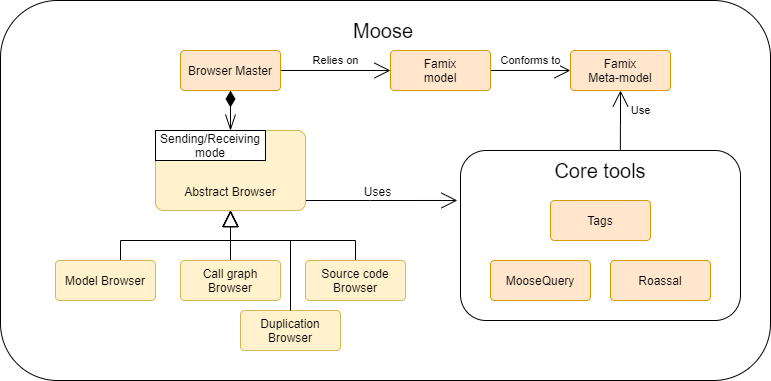
\includegraphics[width=0.7\linewidth]{./figures/architecture.png}
  \caption{Architecture de la suite d'outils}
  \label{fig:applicationArchitecture}
  \end{center}
  \vspace{-0.3cm}
\end{figure}

La \figref{applicationArchitecture} montre l'architecture globale de la suite d'outils.
L'architecture globale de la suite d'outils est principalement composée d'un \browserMaster et des navigateurs.
Le tout s'exécute sur une instance d'un modèle Famix. 
Il a été pensé dans le but de facilité l'expérience du développeur dans les différentes activités de la rétro-ingénierie logiciel.
Le \browserMaster est responsable de l'échange d'information entre les navigateurs.
Il est au courant de tous les navigateurs ouvert. 
Il se charge de notifier tous les navigateurs ouverts en cas d'événement.

Chaque navigateur fonction sur une entité du modèle  local a lui.
Cette entité peut être une seule entité ou un groupe d'entité.
Il navigateur est peut émettre ou recevoir un événement. 
\paragraph{émission d'événement:} l'émission d'un événement par un navigateur est gouverner par son mode de propagation.
En mode de propagation active, le navigateur émet un événement pour publier son entité courant a chaque fois que l'entité change.
Dans le contraire, l'entité courant est gardée localement.

\paragraph{réception d'événement : } le comportement d'un navigateur a la réception d'un événement dépend du mode de réception de ce dernier.
Ainsi, chaque navigateur possède trois modes de réception d'événement. 
Il s'agit des modes (1) \textit{follow}: le navigateur change remplace son entité courant par l'entité reçu via l'événement.
(2) \textit{highlight}: le navigateur cherche l'entité reçu via l'événement dans son entité courant, s'il le trouve, il le colorie.
(3) \textit{ignore}: le navigateur ne fait rien à la réception de l'événement.

Tous les navigateurs présentent un bouton qui indique sont mode d'émission d'événement, et trois boutons qui indiquent sont mode de réception d'événement.

\subsubsection{Nivagateur de modèle}
\begin{figure}[htbp]
  \begin{center}
  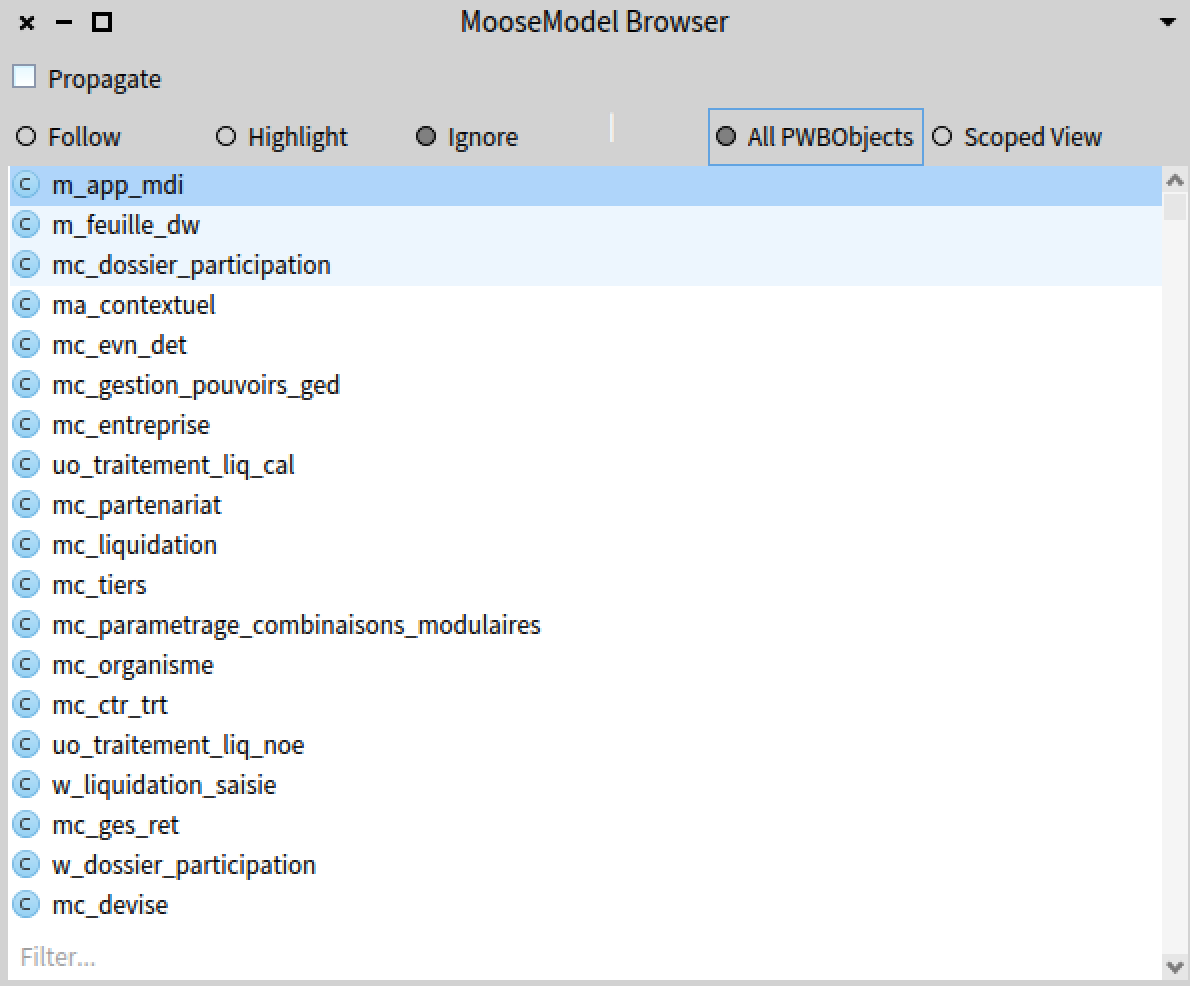
\includegraphics[width=0.6\textwidth]{./figures/modelBrowser.png}
  \caption{Navigateur de modèle}
  \label{fig:modelBrowser}
\end{center}
\vspace{-0.3cm}
\end{figure}
Le navigateur de modèle comme la montre la \figref{modelBrowser} outre la partie commune a touts les navigateurs, comporte deux boutons (\textit{All PWBObjects}, \textit{Scoped View}), un contenu et un champ de recherche.

Le contenu navigateur présente par défaut la liste des entités que contient l'entité courant du navigateur. 
L'utilisateur peut décider de se concentrer sur un certain nombre d'entités. Dans ce cas, il les sélectionne et il active le bouton \textit{Scoped View}.
Pour le moment le navigateur de modèle est juste une liste. Mais il est prévu de l'étendre.

Le champ de recherche du navigateur permet à l'utilisateur d'écrire une requête de recherche sur son entité Famix courante.
Cette entité est pour la plupart du temps un groupe d'entité Famix.
Cette requête peut être lexicale, sous forme de simple chaîne pour une recherche lexicale, ou structurelle.
Par exemple, si l'utilisateur recherche \textit{include : FamixPWBAttribute}, le résultat sera toutes les entités contenant des FamixPWBAttribute (attributs Powerbuilder).

\subsubsection{navigateur de graph d'appel}
\begin{figure}[htbp]
  \begin{center}
  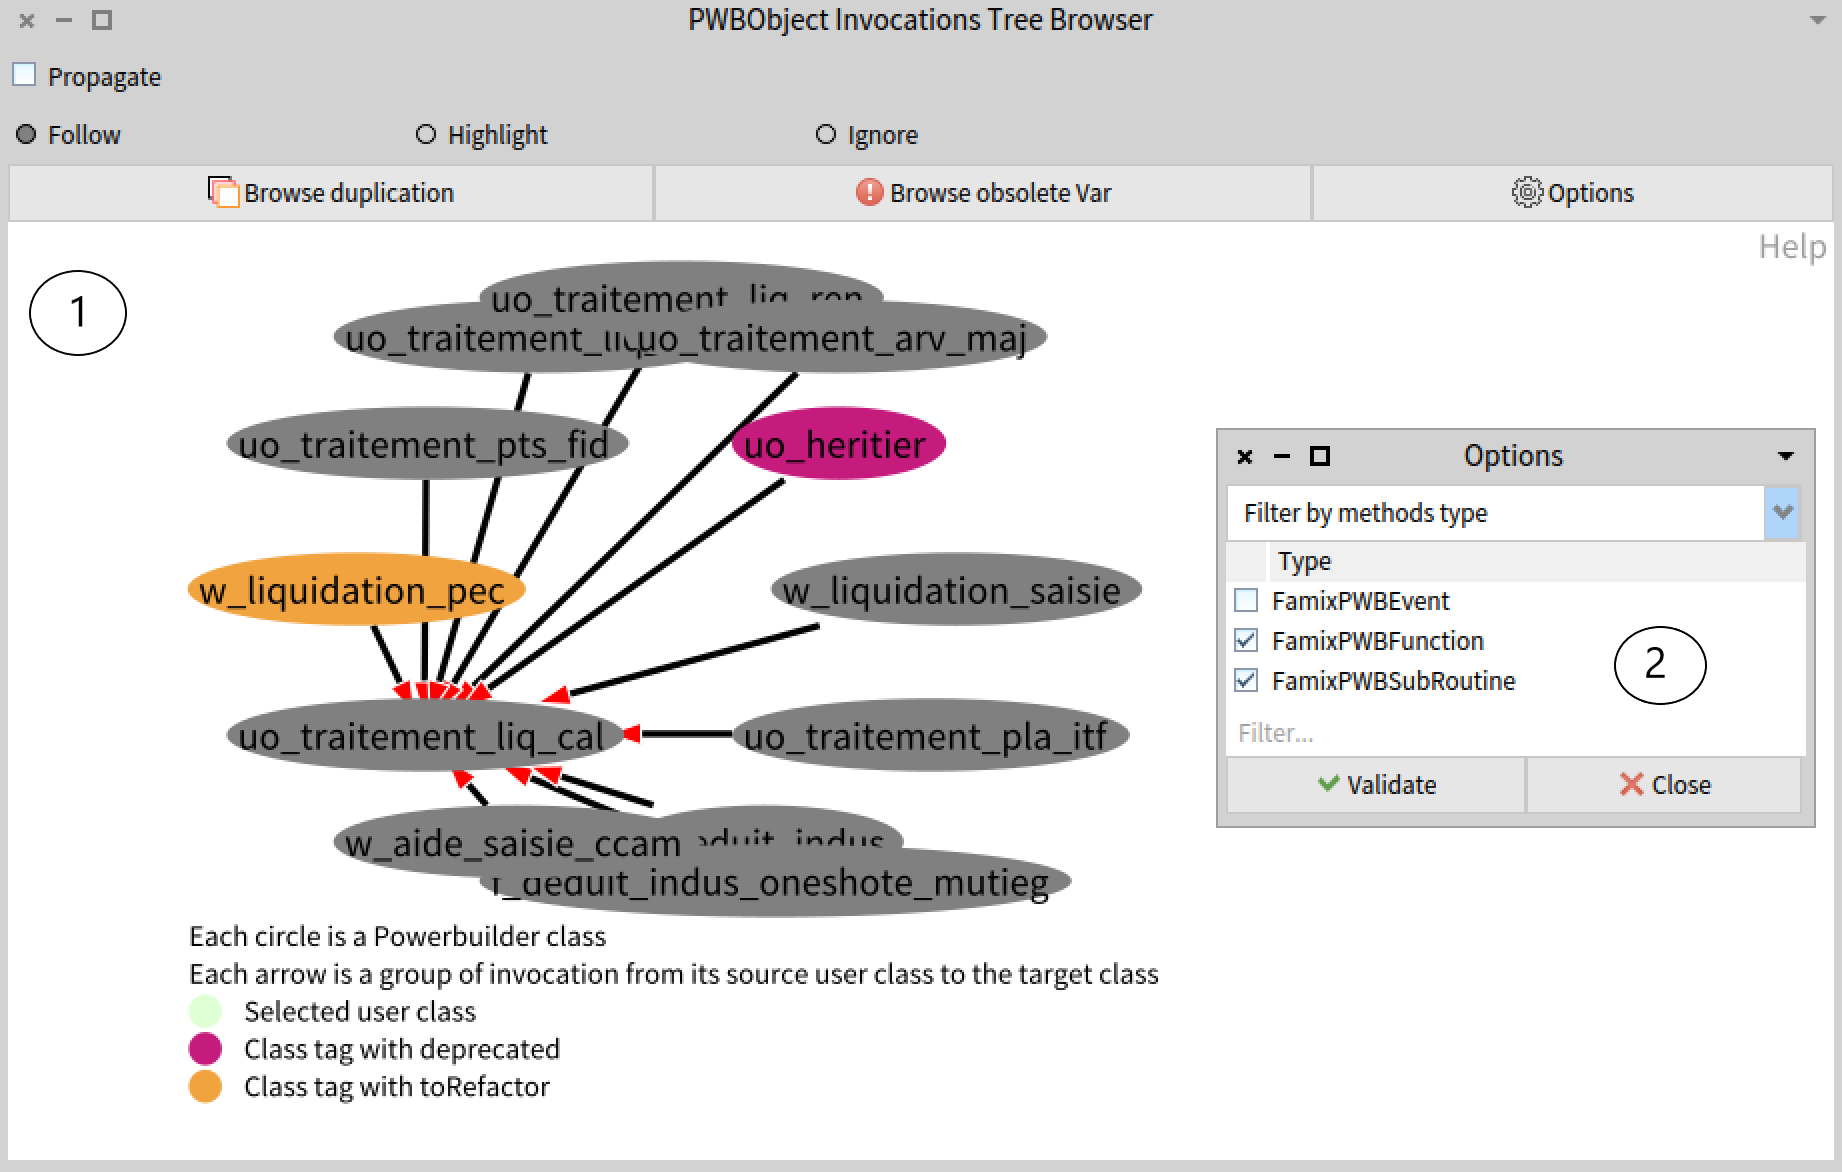
\includegraphics[width=0.9\textwidth]{./figures/callGraphBrowser.png}
  \caption{Graphe d'appel avec l'option de reduction de complexité du graphe}
  \label{fig:graphAppel}
\end{center}
\vspace{-0.3cm}
\end{figure}
La \figref{graphAppel} donne un aperçu du graphe d'appel avec les options.  
 La fenêtre (1) de ce outil permet principalement de visualiser sous forme d'un graphe les entités qui utilisent l'entité courant du navigateur.
Les nœuds représentent les entités. Les flèches représentent l'ensemble des utilisations entre deux entités.
Le sens de la flèche indique le sens des utilisations.
En effet pour un système large comme Izy Protect par exemple, ce graphe peut rapidement devenir illisible. 
Pour palier à ce problème, l'outil intègre un panel d'option( la fenêtre (2) de la \figref{graphAppel}) qui permet de filtrer le graphe par type d'entité a l'origine des appels.
Afin de donner plus de contexte aux développeurs, quand il glisse la souris sur une flèche, un popup lui montre toutes les utilisations avec leur code source.

Le navigateur de graphe d'appel permet aussi aux développeurs de marquer les entités afin de lui ajouter une information qu'on ne peut pas extraire directement du code source.
Une connaissance qui ressort de l'expérience du développeur sur le système.
\subsubsection{navigateur de Code mort}
\begin{figure}[htbp]
  \begin{center}
  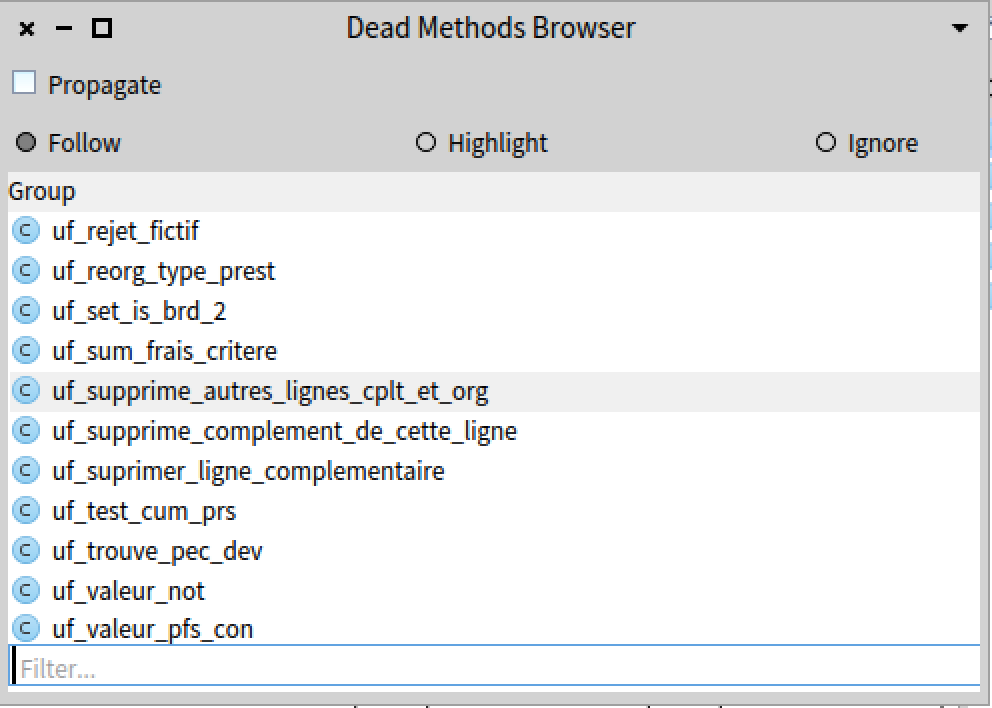
\includegraphics[width=0.5\textwidth]{./figures/deadMethodBrowser.png}
  \caption{navigateurde code mort}
  \label{fig:deadMethodBrowser}
\end{center}
\vspace{-0.3cm}
\end{figure}
La \figref{deadMethodBrowser} montre le navigateur de code mort.
Ce navigateur pressent pour le moment les méthodes de l'entité courant du navigateur qui le sont jamais appelé dans le système et les que ces méthodes appels.

\subsubsection{navigateur de code dupliqué}
\begin{figure}[htbp]
  \begin{center}
  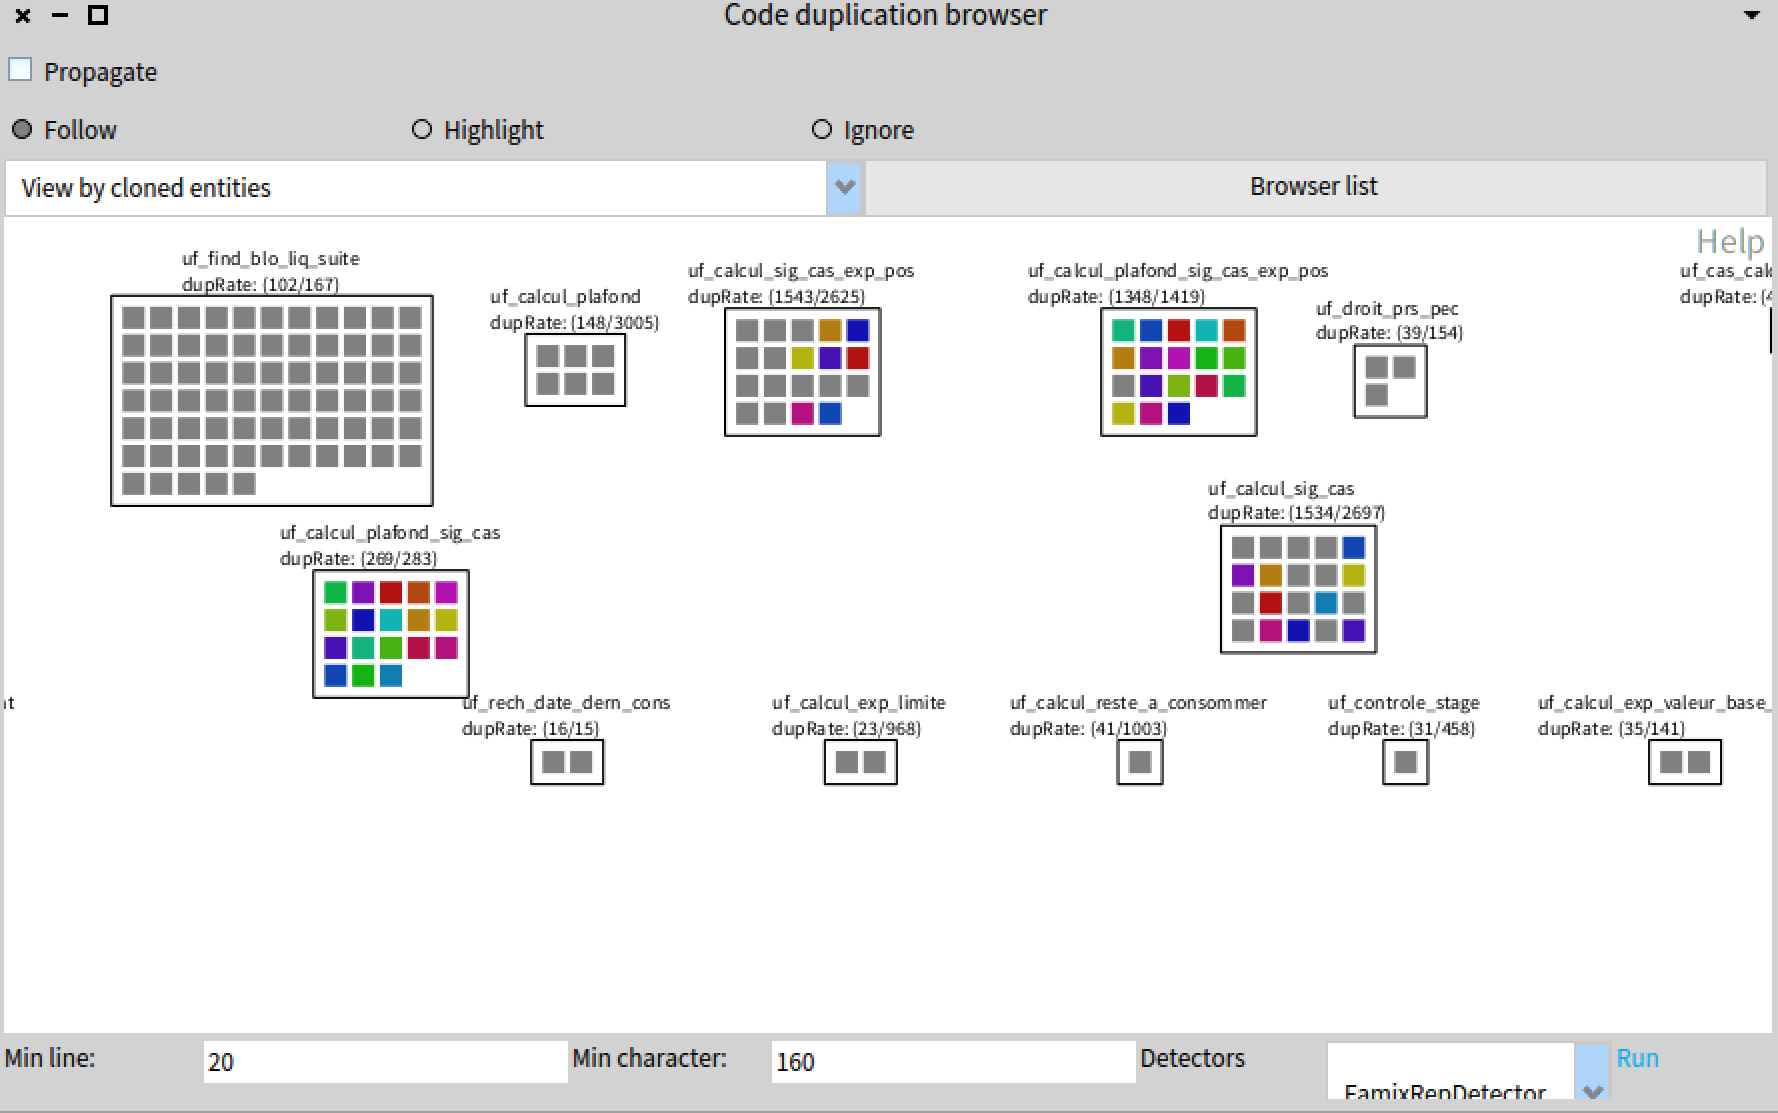
\includegraphics[width=0.9\textwidth]{./figures/duplicationBrowser.png}
  \caption{navigateur de code dupliqué}
  \label{fig:duplicationBrowser}
\end{center}
\vspace{-0.3cm}
\end{figure}
La \figref{duplicationBrowser} présent le navigateur de code dupliqué. Les carrés externes représentent les entités qui présentent de clone.
Dans le cas de la \figref{duplicationBrowser} c'est des méthodes. 
Les carrés internes représentent les clones que présente une entité.
Les clones sont représentés de façon de ce que l'utilisateur puis facilement l'inspecter.
Il utilise actuellement un algorithme de détection basé sur l'égalité strict des chaînes de caractères \citep{Duca99b}. 
Cet algorithme peut être remplacé par un algorithme plus sophistiqué pour détecter les doublons \citep{Roy07a}. 

Supposons deux entités \textit{e1} et \textit{e2} qui présentent de clones en commun.
Quand l'utilisateur clique sur \textit{e1}, les clone de \textit{e1} prennent des couleurs différentes.
Les clones que \textit{e1} à en commun avec \textit{e2}, dans \textit{e2} prennent les mêmes couleurs que leurs semblables dans \textit{e1}.
Cela permet de voir plus facilement quelles entités ont de code en commun et de comparer les codes sources dans le navigateur de code que je présenterai dans la suite. 

\subsubsection{Navigateur de code source}
\begin{figure}[htbp]
  \begin{center}
  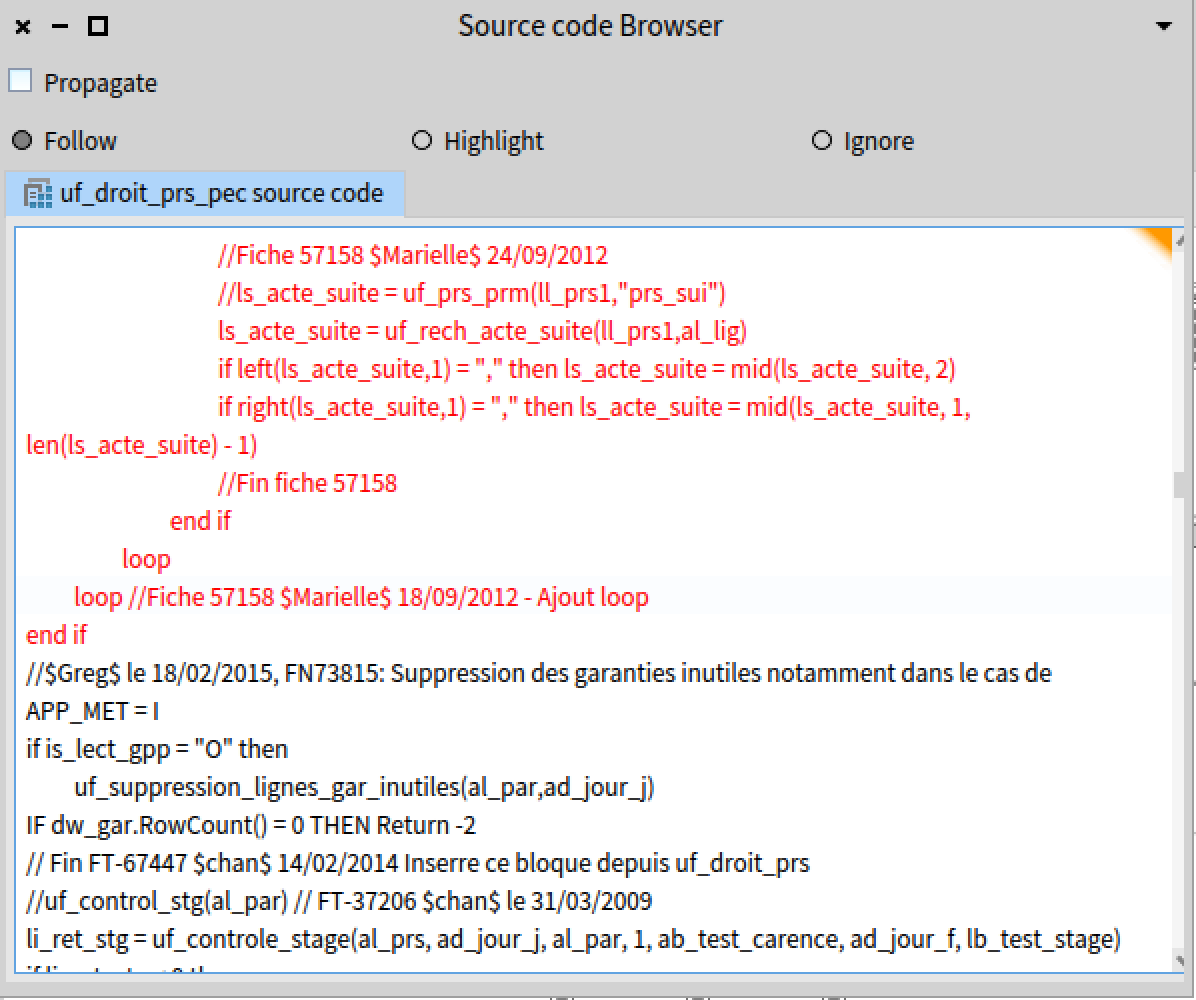
\includegraphics[width=0.7\textwidth]{./figures/sourceCodeBrowser.png}
  \caption{navigateur de code dupliqué}
  \label{fig:sourceCodeBrowser}
\end{center}
\vspace{-0.3cm}
\end{figure}
La \figref{sourceCodeBrowser} présente le navigateur de code source. 
Ce navigateur est une fenêtre qui affiche le code source de l'entité courant.
En particulier dans le cadre d'un fragment dupliqué, le code source de l'entité qui contient ce fragment est affiché normalement sauf que la partie du code qui représente le fragment dupliqué est en rouge comme sur la \figref{sourceCodeBrowser}

\section{Future travaux}
\label{sec:roadmap}
Toutes les outils présentes ci-dessus sont conçus dans le but de nettoyer le code de visualiser l'interaction entre les différentes classe d'Izy Protect.
Par contre les développeurs ne l'ont pas encore utilisé dans leur quotidien.
Dans ce sens, j'identifie la validation de ces outils dans la suite mes travaux.

D'un autre côté, l'entreprise prévoit de migrer une partie du système dans une architecture orienté service. 
Les développeurs ont donc exprimé le besoin d'extraire des logiques métier du code.
Plusieurs travaux sont présentés dans la literature dans ce sens en particulier \cite{Lei05a} qui se base sur l'analyse statique des interaction des fonctions avec les variables pour extraire les logiques metier d'un systemes patrimonial. 
Je souhaite combiner cette méthode avec la méthode proposée \cite{anqu19a} pour proposer un outil d'extraction de logique métier dans les systèmes patrimoniaux.

Je mettrai en place et j'étudierai l'impact du DevOps à la CIM. 

\section{Publications}

Les articles soumis dans le cadre de cette thèse sont :
\begin{enumerate}
\item Improving practices in a medium Franch company : First step (\citet{Houe20a})
\item Towards a Versatile Reverse Engineering Tool Suite ( \citet{Houe20b})

\end{enumerate}

\section{Formations}
Voici la liste des formations que j'ai assistées :
\begin{itemize}
\item Les fondamentaux du management d’équipe Session 1 (Ecole doctorale)
\item Gestion de conflit (CIM) 
\item Formation Propriété intellectuelle au service des doctorants tronc commun (Ecole doctorale)
\item Intelligence économique et dynamique de l'innovation (Ecole doctorale)
\item Communiquer en Anglais - Niveau confirmé - Stage intensif (Ecole doctorale)
\end{itemize}

\section{Projet professionnel}
En ce qui concerne mon projet professionnel, je souhaite continuer dans l'enseignement supérieur : donner des cours et continuer dans la recherche.
Je pense la reengenierie des système est un axe de recherche ou beaucoup de travaux intéressant sont mener. Néanmoins il reste à faire et je souhaite contribuer a cela.
Toutefois, je ne me refuse pas l'idée de démarrer une start-up a l'issue de ma thèse ou travailler dans une entreprise.

\footnotesize{
  %\bibliographystyle{alpha}
  % natbib 
 \bibliographystyle{plainnat}
\bibliography{rmod,others,nextPubli}
}

\end{document}